\chapter{Installation Guide} \label{app:installation}

A installation guide\footnote{Linux-based operation system is preferred} for both \CodeName and BDAE including an available test and example suite with samples such as the ones explained in section \ref{sec:examples} in the analysis phase of \CodeName. The source code archive\footnote{\texttt{<project path>/src/}} of the combined project will onwards be referenced as \texttt{src/} and assumed to be fetched from the repository.

\begin{enumerate}
	\item Install \CodeName:
	
	\begin{lstlisting}[numbers=none, backgroundcolor=\color{sourcebackground}, rulecolor=\color{sourcebackground}, framextopmargin=5pt, framexbottommargin=5pt, frame=tb, xrightmargin=15pt]
	cd src/sofa-project
	bash install.sh
	\end{lstlisting}
	\vspace*{-6mm}
	\item Install BDAE:
	
	\begin{lstlisting}[numbers=none, backgroundcolor=\color{sourcebackground}, rulecolor=\color{sourcebackground}, framextopmargin=5pt, framexbottommargin=5pt, frame=tb, xrightmargin=15pt]
	cd src/bdae-project
	bash install.sh
	\end{lstlisting}
	\vspace*{-6mm}
	\item Create new empty project directory\footnote{Will ahead be denoted as \texttt{example/}}.
	\item Duplicate and modify the system configuration file to fit the purpose:
	
	\begin{lstlisting}[numbers=none, backgroundcolor=\color{sourcebackground}, rulecolor=\color{sourcebackground}, framextopmargin=5pt, framexbottommargin=5pt, frame=tb, xrightmargin=15pt]
	cd example
	cp $SOFA_HOME/sofa/sofa.cfg my_sofa.cfg
	vim my_sofa.cfg
	\end{lstlisting}
	
	\item Enable local SSH\footnote{Extra step on macintosh-based systems available here: \url{http://www.techradar.com/how-to/computing/apple/how-to-enable-ssh-on-your-mac-1305644}} to fully utilize the supplied boot-scripts (explained and exemplified in appendix \ref{app:execution}):
	
	\begin{lstlisting}[numbers=none, backgroundcolor=\color{sourcebackground}, rulecolor=\color{sourcebackground}, framextopmargin=5pt, framexbottommargin=5pt, frame=tb, xrightmargin=15pt, commentstyle=\color{bashcommetcolor}]
	cd ~/.ssh/
	touch authorized_keys
	cat id_rsa.pub > authorized_keys
	
	# Verify by ssh to localhost
	ssh localhost
	\end{lstlisting}
	\vspace*{-6mm}
	\item Install following extra Python 2.7 packages to run all BDAE examples, located in \texttt{\$BDAE\_HOME/examples}:

	\begin{lstlisting}[numbers=none, backgroundcolor=\color{sourcebackground}, rulecolor=\color{sourcebackground}, framextopmargin=5pt, framexbottommargin=5pt, frame=tb, xrightmargin=15pt, commentstyle=\color{bashcommetcolor}, showstringspaces=false]
	# Prerequisite for text.py
	pip install ntlk
	python -c "import nltk; nltk.download('punkt')"
	
	# Prerequisite for avs5m.py
	pip install tifffile
		
	# Prerequisite for NetCDF pop.py
	pip install netCDF4
	\end{lstlisting}
	\vspace*{-6mm}
	\item[$\bullet$] {\sffamily\textbf{NOTE:}} To uninstall \CodeName and BDAE, use following two commands:
	\begin{lstlisting}[numbers=none, backgroundcolor=\color{sourcebackground}, rulecolor=\color{sourcebackground}, framextopmargin=5pt, framexbottommargin=5pt, frame=tb, xrightmargin=15pt, commentstyle=\color{bashcommetcolor}, showstringspaces=false]
	cd src/
	bash clean.sh sofa
	bash clean.sh bdae		
	\end{lstlisting}
\end{enumerate}


\chapter{Execution Guide} \label{app:execution}
Assuming the installation guide at appendix \ref{app:installation} is completed.

\begin{itemize}
	\item {\sffamily\textbf{NOTE:}} A general boot script is provided as part of the installation of \CodeName and can succesfully initialize all three type of server. The script requires that the SSH (explained in appendix \ref{app:installation}) is properly configured on each machine.
	\begin{lstlisting}[numbers=none, backgroundcolor=\color{sourcebackground}, rulecolor=\color{sourcebackground}, framextopmargin=5pt, framexbottommargin=5pt, frame=tb, xrightmargin=15pt, commentstyle=\color{bashcommetcolor}, showstringspaces=false, deletendkeywords={file, list}]
	cd $SOFA_HOME/
	
	# General pattern for the boot script
	bash boot.sh <path to cfg file> <state>
	\end{lstlisting}
	\vspace*{-6mm}

	\item Gateway example:
	\begin{lstlisting}[numbers=none, backgroundcolor=\color{sourcebackground}, rulecolor=\color{sourcebackground}, framextopmargin=5pt, framexbottommargin=5pt, frame=tb, xrightmargin=15pt, commentstyle=\color{bashcommetcolor}, showstringspaces=false]
	bash boot.sh example/my_sofa.cfg gateway storage
	\end{lstlisting}
	\vspace*{-6mm}
	
	\item Storage example:
	\begin{lstlisting}[numbers=none, backgroundcolor=\color{sourcebackground}, rulecolor=\color{sourcebackground}, framextopmargin=5pt, framexbottommargin=5pt, frame=tb, xrightmargin=15pt, commentstyle=\color{bashcommetcolor}, showstringspaces=false]
	bash boot.sh example/my_sofa.cfg storage
	\end{lstlisting}
	\vspace*{-6mm}
	
	\item Monitor example:
	\begin{lstlisting}[numbers=none, backgroundcolor=\color{sourcebackground}, rulecolor=\color{sourcebackground}, framextopmargin=5pt, framexbottommargin=5pt, frame=tb, xrightmargin=15pt, commentstyle=\color{bashcommetcolor}, showstringspaces=false]
	bash boot.sh example/my_sofa.cfg monitor storage gateway
	\end{lstlisting}	
\end{itemize}

Note that the \texttt{state} parameter is a list of node types, where the first element is the kind that the current node will adapt. The rest of the optional element in the list is the kind of nodes that the current one will have an awareness of.
\newline

The nodes are bootable by the python daemon too, in the case of misconfigured SSH or other reasons:
\vspace*{2mm}

\begin{lstlisting}[numbers=none, backgroundcolor=\color{sourcebackground}, rulecolor=\color{sourcebackground}, framextopmargin=5pt, framexbottommargin=5pt, frame=tb, xrightmargin=15pt, commentstyle=\color{bashcommetcolor}, showstringspaces=false, deletendkeywords={file, list}]
	python $SOFA_HOME/sofa/boot.py <unique node index> <path to cfg file> <state>
\end{lstlisting}	

{\sffamily\textbf{NOTE:}} A Pyro4 NameService\footnote{Command: \texttt{pyro4-ns}}, one gateway and one storage node is a bare minimum to get started.

\chapter{Application Screenshots} \label{chp:app-screenshots}

\begin{figure*}[h!]
	\centering
  	\begin{minipage}[b]{0.4\textwidth}
    		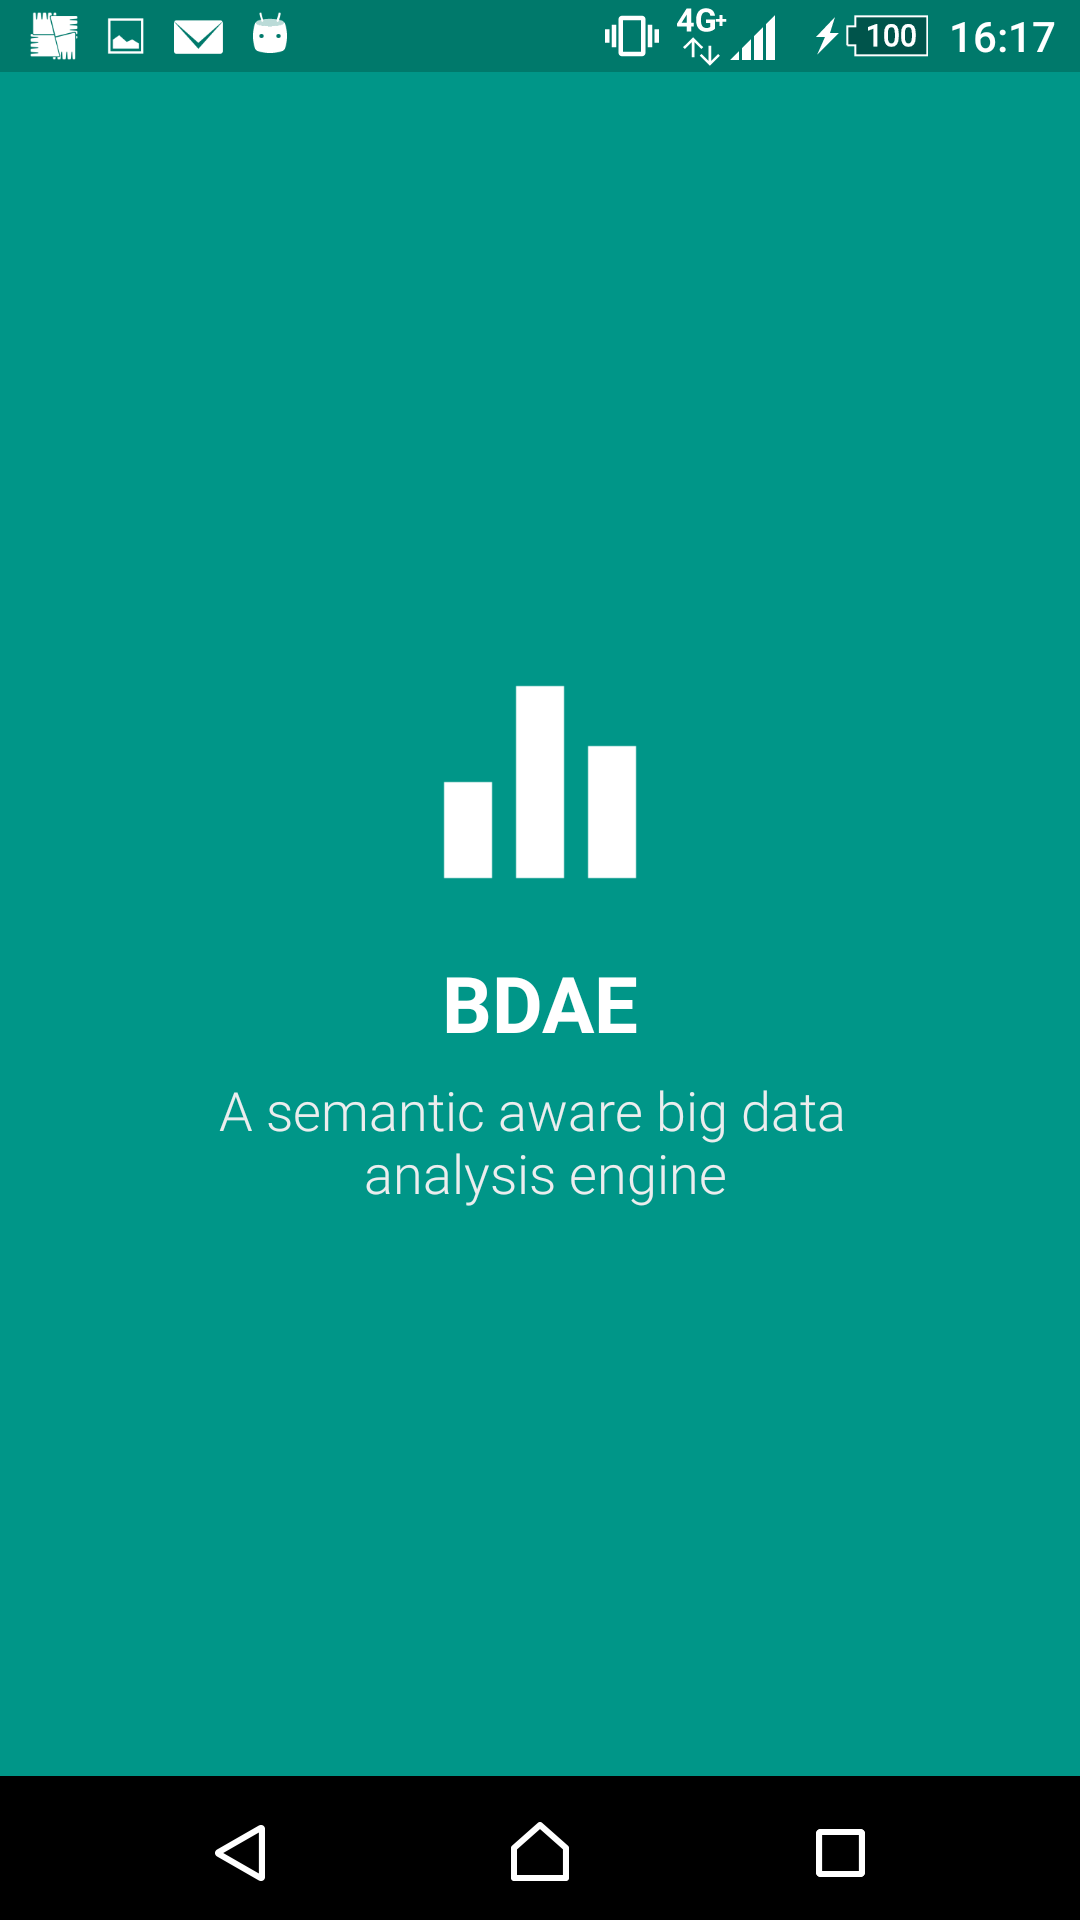
\includegraphics[width=\textwidth]{img/loadingscreen.png}
    \end{minipage}
  	\hfill
  	\begin{minipage}[b]{0.4\textwidth}
    		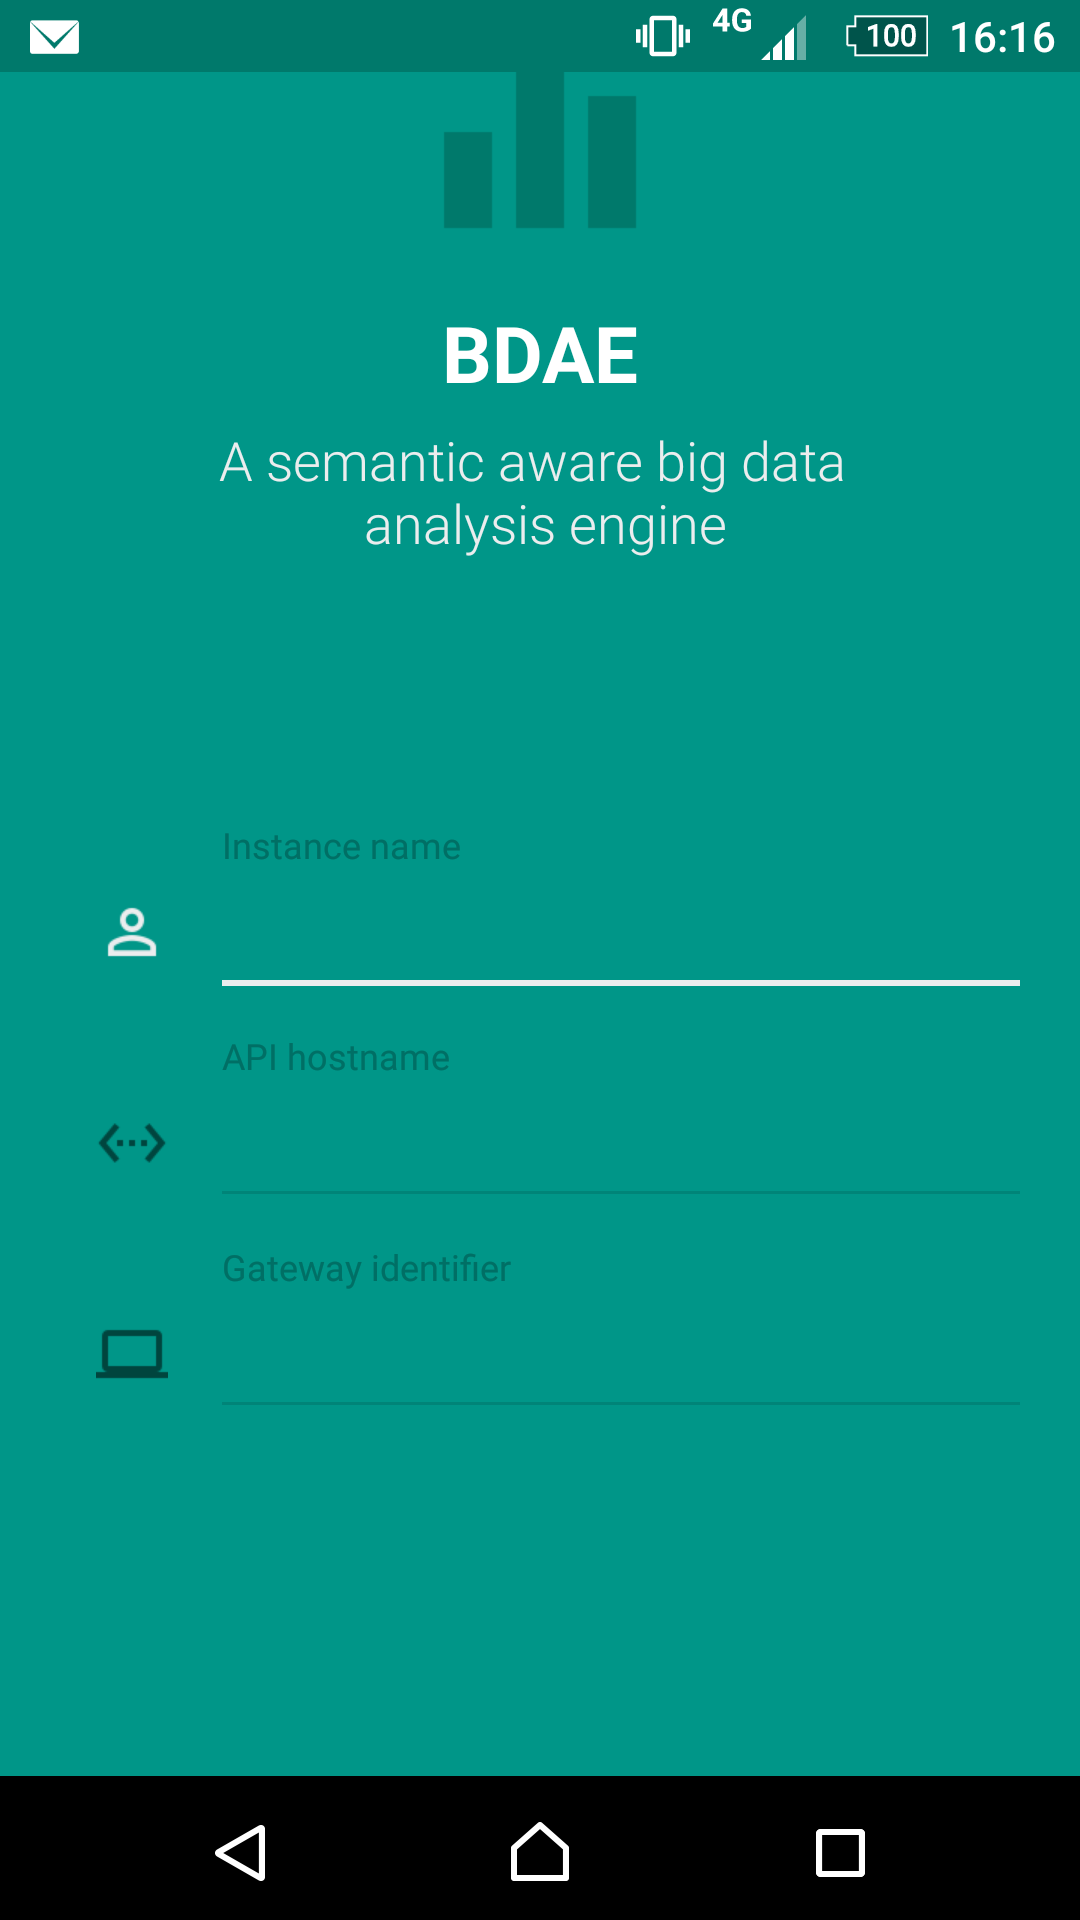
\includegraphics[width=\textwidth]{img/information.png}
  	\end{minipage}
  	\caption[]{Loading screen animated into the required information screen.}
\end{figure*}

\begin{figure*}[h!]
	\centering
  	\begin{minipage}[b]{0.4\textwidth}
    		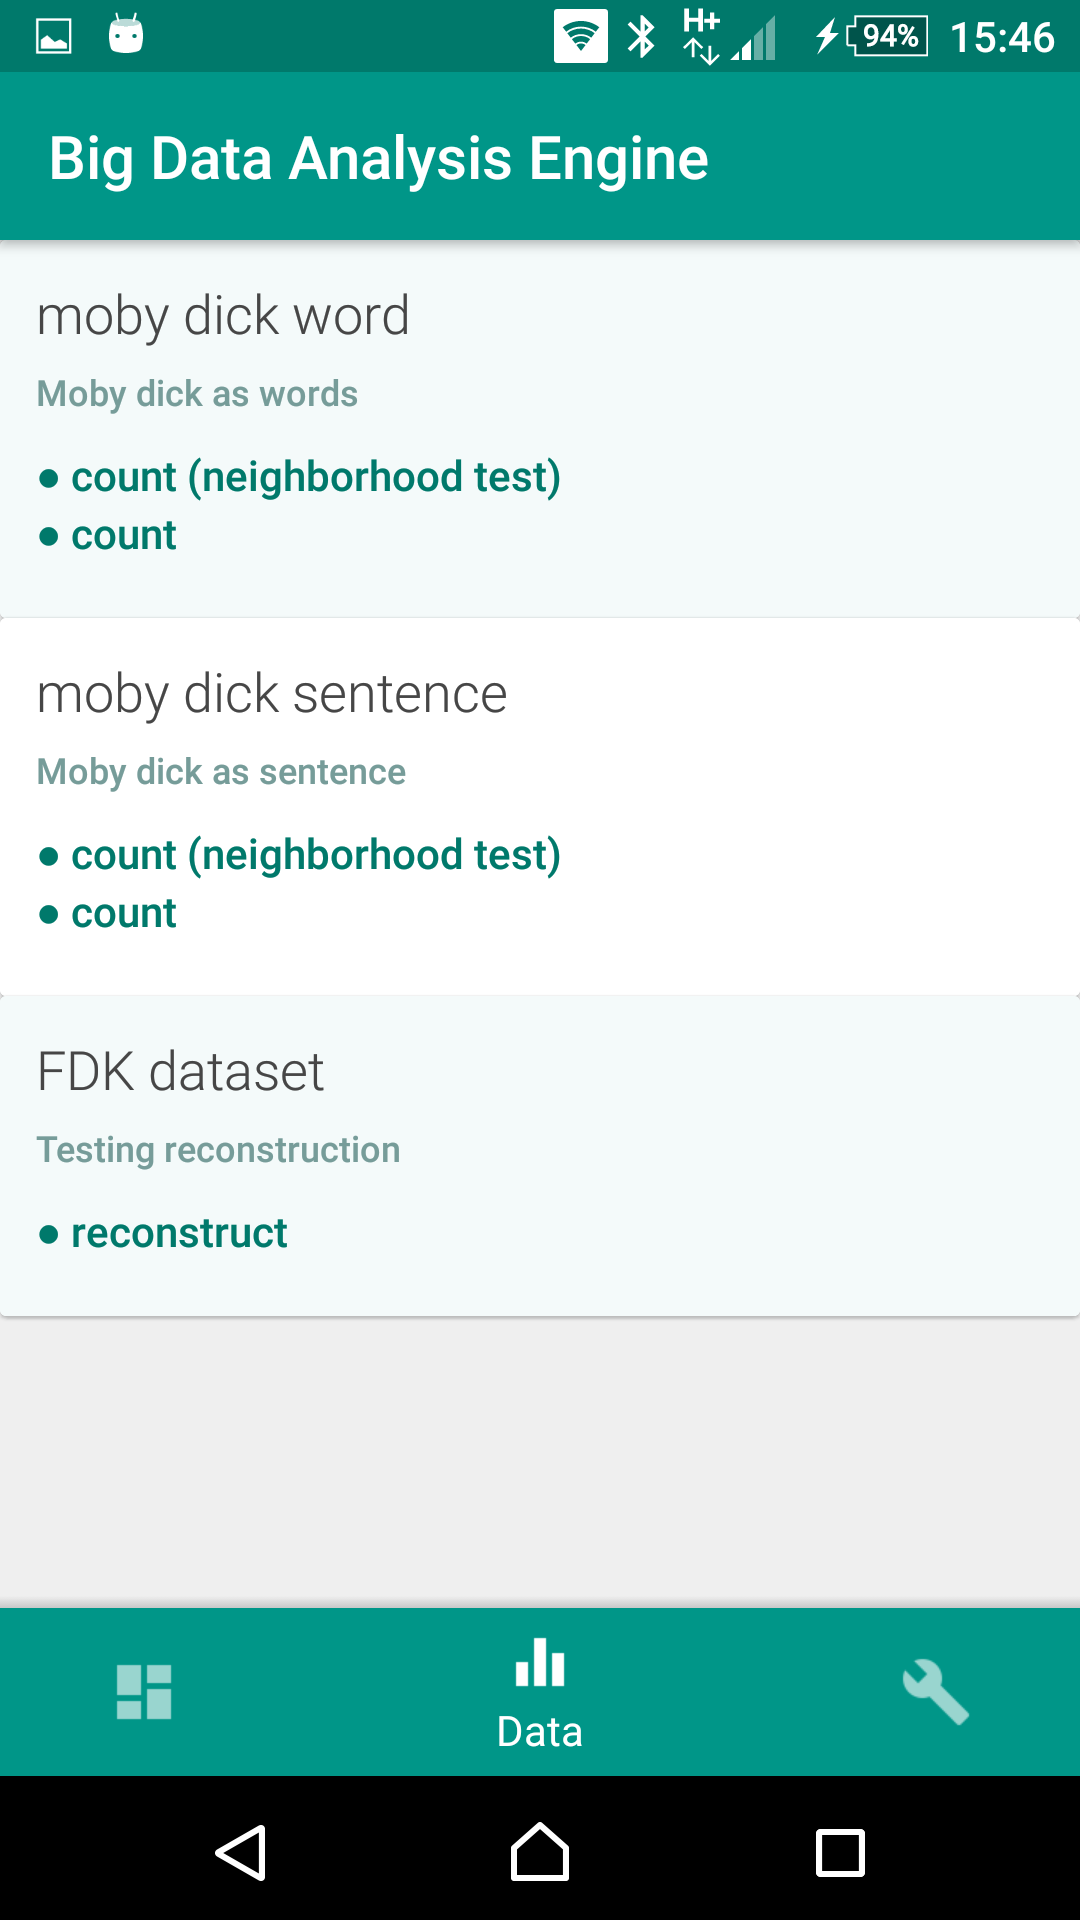
\includegraphics[width=\textwidth]{img/datasets.png}
   	  	\caption[]{List of available datasets and their associated operations.}
    \end{minipage}
  	\hfill
  	\begin{minipage}[b]{0.4\textwidth}
    		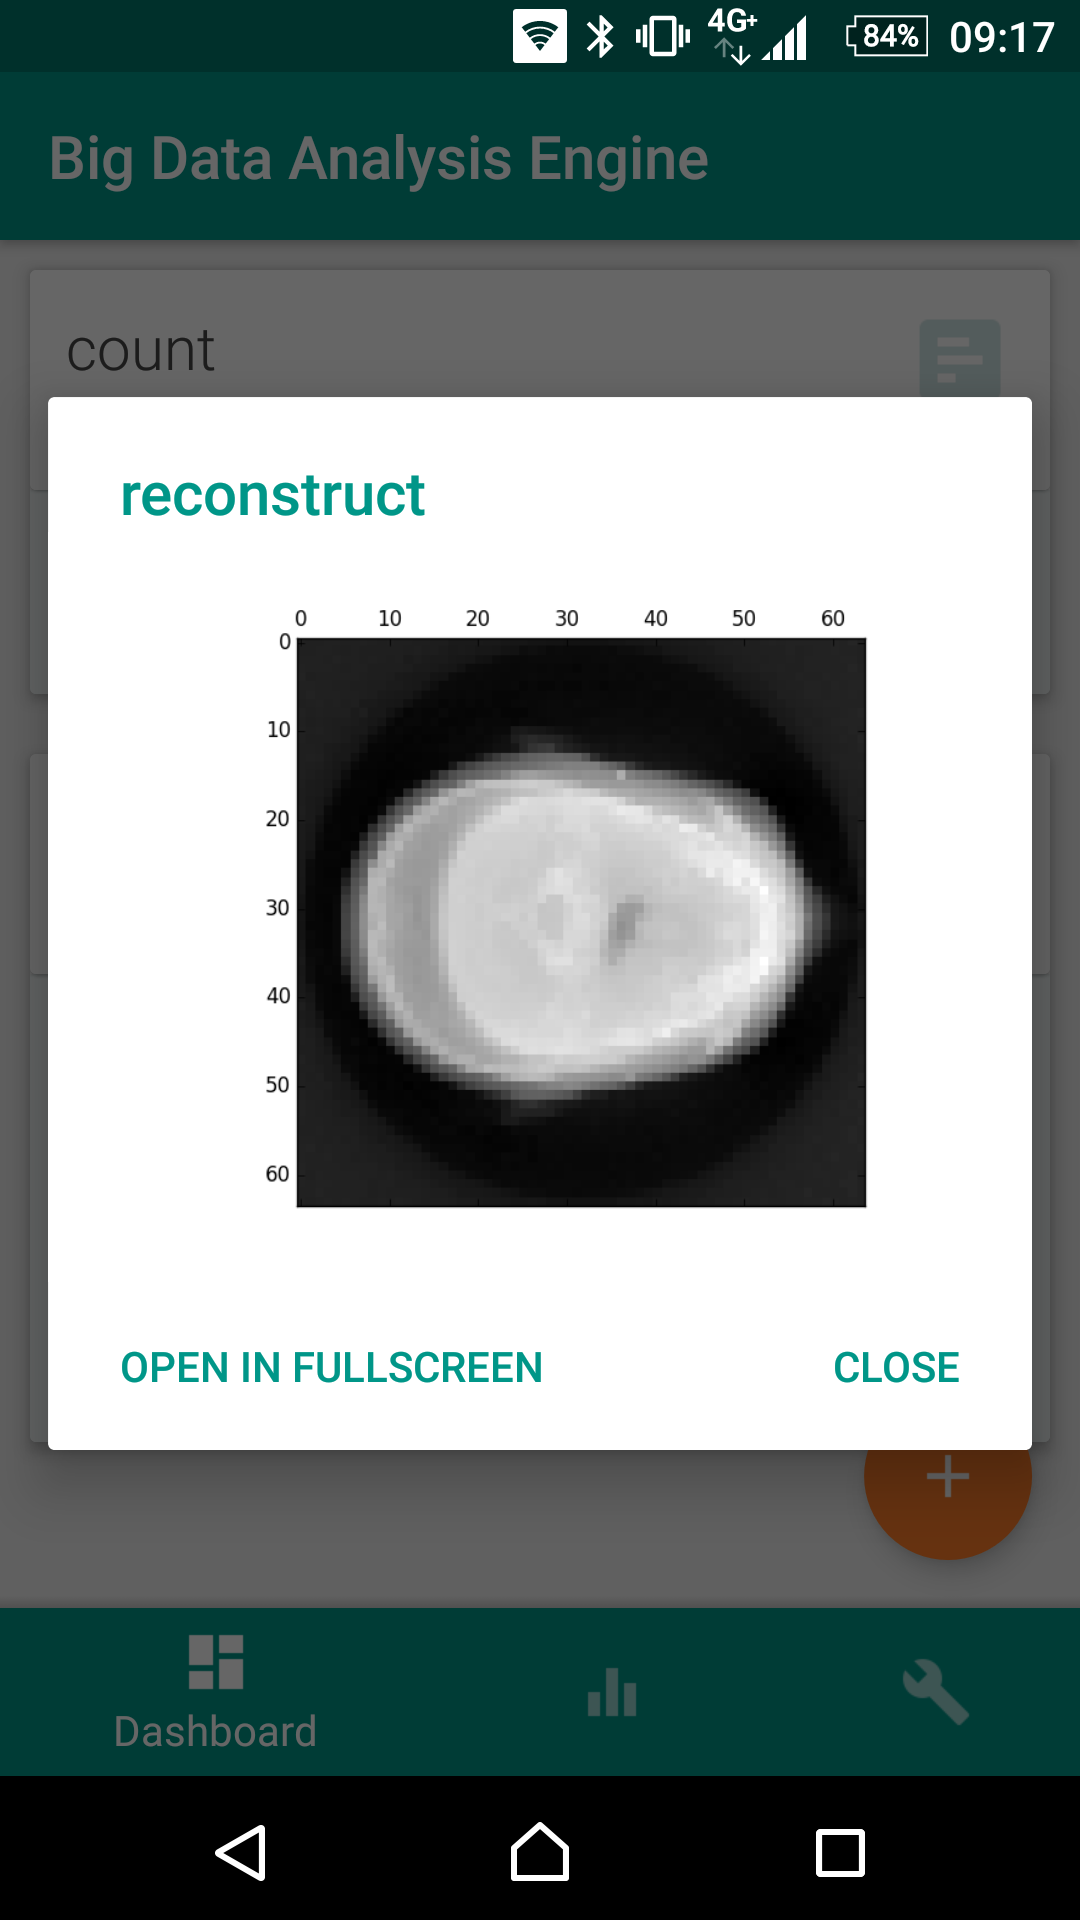
\includegraphics[width=\textwidth]{img/result.png}
    		\caption[]{A dialog displaying the result of a CT reconstruction operation.}
  	\end{minipage}
\end{figure*}

\chapter{Benchmark Graphs}
\section{CT reconstruction} \label{app:fdk}
\begin{figure}[h!]
	\centering
	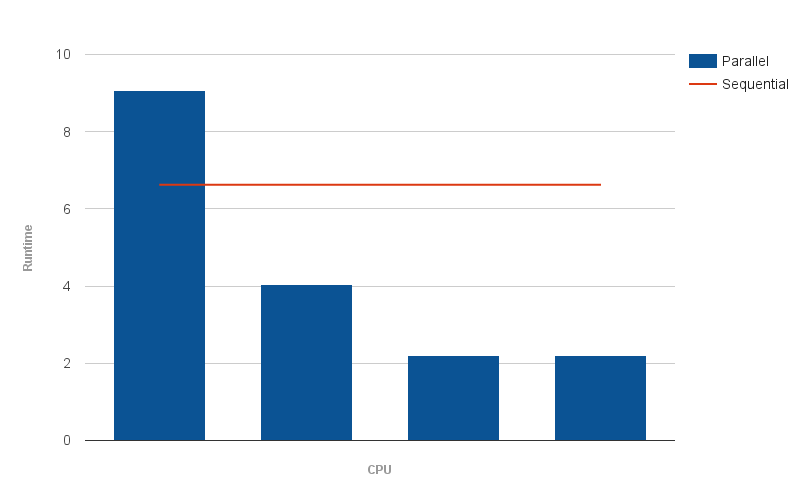
\includegraphics[scale=0.4]{img/fdk-64.png}
	\caption[]{Execution time of the 64x64x64 voxels dataset. \label{fig:fdk-64}}
\end{figure}

\begin{figure}[h!]
	\centering
	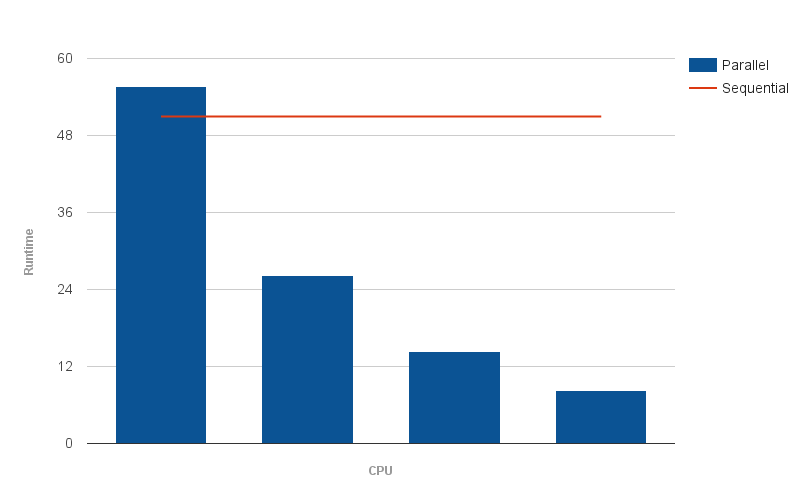
\includegraphics[scale=0.4]{img/fdk-128.png}
	\caption[]{Execution time of the 128x128x128 voxels dataset. \label{fig:fdk-128}}
\end{figure}

\begin{figure}[h!]
	\centering
	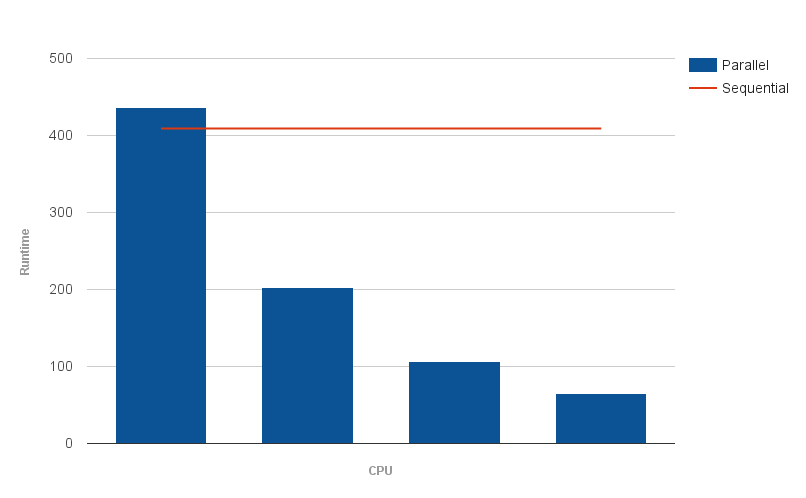
\includegraphics[scale=0.4]{img/fdk-256.png}
	\caption[]{Execution time of the 256x256x256 voxels dataset. \label{fig:fdk-256}}
\end{figure}

\chapter{Hadoop Source Code Example}
\definecolor{pblue}{rgb}{0.13,0.13,1}
\definecolor{pgreen}{rgb}{0,0.5,0}
\definecolor{pred}{rgb}{0.9,0,0}
\definecolor{pgrey}{rgb}{0.46,0.45,0.48}

\section{Map} \label{sec:hadoop-map}
\begin{lstlisting}[language=Java, commentstyle=\color{pgreen}, keywordstyle=\color{pblue}, stringstyle=\color{pred},basicstyle=\fontsize{6}{5}\selectfont\ttfamily, xleftmargin=0.8cm]
package com.cloudera.example;

import org.apache.hadoop.io.IntWritable;
import org.apache.hadoop.io.LongWritable;
import org.apache.hadoop.io.Text;
import org.apache.hadoop.mapreduce.Mapper;

import java.io.IOException;

public class LogEventParseMapper extends Mapper<LongWritable, Text, Text, IntWritable> {
    
    enum Level { TRACE, DEBUG, INFO, WARN, ERROR, FATAL };

    @Override
    public void map(LongWritable key, Text value, Context context)
            throws IOException, InterruptedException {

        String line = value.toString();

        // ignore empty lines
        if (line.trim().isEmpty()) {
            return;
        }
        String[] fields = line.split(" ");

        // ensure this line is not malformed
        if (fields.length <= 3) {
            return;
        }

        String levelField = fields[3];
        for (Level level : Level.values()) {
            String levelName = level.name();
            if (levelName.equalsIgnoreCase(levelField)) {
                context.write(new Text(levelName), new IntWritable(1));
            }
        }
    }
}
\end{lstlisting}
\newpage
\section{Reduce} \label{sec:hadoop-reduce}
\begin{lstlisting}[language=Java, commentstyle=\color{pgreen}, keywordstyle=\color{pblue}, stringstyle=\color{pred},basicstyle=\fontsize{6}{5}\selectfont\ttfamily, xleftmargin=0.8cm]
package com.cloudera.example;

import java.io.IOException;

import org.apache.hadoop.io.IntWritable;
import org.apache.hadoop.io.Text;
import org.apache.hadoop.mapreduce.Reducer;

public class LogEventSumReducer extends Reducer<Text, IntWritable, Text, IntWritable> {

    @Override
    public void reduce(Text key, Iterable<IntWritable> values, Context context) 
            throws IOException, InterruptedException {

        // used to count the number of messages for this event type
        int sum = 0;
        // increment it for each new value received
        for (IntWritable value : values) {
            sum += value.get();
        }

        // Our output is the event type (key) and the sum (value)
        context.write(key, new IntWritable(sum));
    }
}
\end{lstlisting}